\appendix
\section{Exact protocol and analysis}\label{exact-protocol-and-analysis}

\subsection{Objective terms, initialization, and parameter
matching}\label{objective-terms-initialization-and-parameter-matching}

The variance and covariance terms of Equation \ref{eq:host} act on the
matrix \(\bar Z^\star\) of batch-and-time-centered active clean targets
with \(N\) rows:

\begin{equation}\mathcal L_{\mathrm{var}}(Z^\star)=\frac1D\sum_{d=1}^{D}\max\!\big(0,\,1-\sqrt{\mathrm{Var}(z^\star_{\cdot d})+\varepsilon}\big),\qquad
\mathcal L_{\mathrm{cov}}(Z^\star)=\frac1D\sum_{d\ne d'}C_{dd'}^2,\quad C=\frac{\bar Z^{\star\top}\bar Z^\star}{N-1}.
\label{eq:vicreg}\end{equation}

All three loss terms have unit weight; there is no selectable
regularizer coefficient. Clean-frame activations, simulator state,
rewards, and corruption labels or masks never enter the recurrent
update; there is no memory teacher and no memory-specific loss. SAS-PC
initialization is \(W_x=I\), \(W_o=W_a=0\), \(b_f=b_m=2\),
\(c_f=c_m=0\), uniform route. The GRU width is fixed once by minimizing
\(|4Dh+3h^2+6h-(2D^2+16D)|\) over hidden sizes \(h\le D\), never re-selected per
task.

\subsection{Immutable identities}\label{immutable-identities}

The frozen execution identities are:

\begin{table}[H]
\centering
\caption{Frozen execution and artifact identities.}
\label{tbl:artifact-identities}
\footnotesize
\begin{tabular}{@{}ll@{}}
\toprule
\textcolor{NVIDIADark}{\textbf{Identity}} & \textcolor{NVIDIADark}{\textbf{Frozen value or SHA-256 prefix}} \\
\midrule
clean worktree at freeze & \texttt{True} \\
protocol SHA-256 & \texttt{357cbe1296926802\ldots} \\
canonical public command-list SHA-256 & \texttt{408051d027c55ae5\ldots} \\
cache-manifest SHA-256 & \texttt{81e3efc64b822741\ldots} \\
cache-sidecar SHA-256 & \texttt{dbc2db0700c30a3e\ldots} \\
artifact-manifest SHA-256 & \texttt{1e3bbcee667a98a6\ldots} \\
cell CSV SHA-256 & \texttt{71144b471acbf88a\ldots} \\
contrast CSV SHA-256 & \texttt{78b804c3acfc433c\ldots} \\
\bottomrule
\end{tabular}
\end{table}

The four-GPU queue was fixed as GPU 0: Acrobot then Stacker; GPU 1:
Manipulator; GPU 2: Quadruped; GPU 3: Swimmer. Every task used optimizer
seeds 18001--18005. The protocol stores all 200 expanded commands and
per-source SHA-256 values; the final analyzer revalidates them before
writing results.

\subsection{Metric phases}\label{metric-phases}

For target time \(t\) and corruption interval \([b,e)\),
\texttt{gap} is \(b\le t<e\), \texttt{deep} is \(b+H\le t<e\),
\texttt{first\_post} is \(t=e\), and \texttt{post} is
\(e<t\le e+H\). The primary held-out metric selects deep and first-post
samples. This selection, the four-corruption average, and all probe
splits were frozen before launch.

\subsection{Crossed bootstrap}\label{crossed-bootstrap}

Let \(\Delta\in\mathbb R^{5\times5}\) contain task-by-seed paired effects. Each draw samples
five task indices and five seed indices independently with replacement,
takes their Cartesian \(5\times5\) submatrix, and averages all entries.
We use 100,000 PCG64 draws with seed 18018 and linear 2.5/97.5
percentiles, preserving the two crossed generalization axes.

\subsection{Comparator identity}\label{comparator-identity}

For each task--seed cell, the recurrent identity is the lower primary
held-out prior NMSE of GRU and SSM; exact ties select GRU. The same
identity supplies deep and clean references; selecting a new best model
separately for those metrics is prohibited. Static/dynamic identity is
selected per cell only for the endpoint noninferiority contrast.

\subsection{Frozen arms and parameter
receipts}\label{frozen-arms-and-parameter-receipts}

The eight arms of Table \ref{tbl:arms} are separately trained; GRU/SSM
update from visual latents only, although the shared predictor remains
action-conditioned. SAS-PC has 33,286--36,614 carrier parameters across
action dimensions; the fixed GRU width gives 35,048. Recurrent carrier
sizes differ by at most 5.29\% and total models by at most 0.09\%.

\section{Registered contrasts in
full}\label{registered-contrasts-in-full}

All eight registered primary contrasts with crossed 95\% and 90\%
intervals and pooled absolute errors:

\begin{table}[H]
\centering
\caption{Registered held-out primary contrasts with 95\% and 90\% crossed bootstrap intervals and pooled candidate/reference NMSE. Deep gap and clean prior use the deep and clean prior-state NMSE against the recurrent envelope; action transport and joint read compare against the no-action and single-read controls; the endpoint envelope is the shrinkage gate of Table \ref{tbl:gate-receipts}.}
\label{tbl:contrast-full}
\footnotesize
\setlength{\tabcolsep}{3.4pt}
\begin{tabular}{@{}lrrrrrr@{}}
\toprule
\textcolor{NVIDIADark}{\textbf{Contrast}} & \textcolor{NVIDIADark}{\textbf{Effect}} & \textcolor{NVIDIADark}{\textbf{95\% CI}} & \textcolor{NVIDIADark}{\textbf{90\% CI}} & \textcolor{NVIDIADark}{\textbf{cells}} & \textcolor{NVIDIADark}{\textbf{tasks}} & \textcolor{NVIDIADark}{\textbf{cand./ref. NMSE}} \\
\midrule
Recurrent envelope & -2.10\% & [-13.35\%, +9.11\%] & [-11.55\%, +7.36\%] & 11/25 & 2/5 & 0.889/0.893 \\
No carrier & +12.44\% & [+3.65\%, +22.43\%] & [+4.89\%, +20.70\%] & 24/25 & 5/5 & 0.889/1.023 \\
Legal integrator & -38.12\% & [-61.38\%, -20.58\%] & [-56.84\%, -21.91\%] & 0/25 & 0/5 & 0.889/0.656 \\
Deep gap & -1.74\% & [-12.95\%, +9.46\%] & [-11.15\%, +7.70\%] & 11/25 & 2/5 & 0.883/0.891 \\
Clean prior & +11.73\% & [+5.82\%, +17.70\%] & [+6.81\%, +16.92\%] & 25/25 & 5/5 & 0.738/0.843 \\
Action transport & +9.48\% & [+2.88\%, +16.09\%] & [+3.94\%, +15.02\%] & 23/25 & 5/5 & 0.889/1.000 \\
Joint read & -5.39\% & [-13.12\%, +0.67\%] & [-11.64\%, +0.07\%] & 6/25 & 1/5 & 0.889/0.855 \\
Endpoint envelope & -1.89\% & [-4.88\%, +0.37\%] & [-4.22\%, +0.00\%] & 6/25 & 0/5 & 0.889/0.876 \\
\bottomrule
\end{tabular}
\end{table}

The table is generated directly from
\texttt{confirmation\_analysis.json}; decisions use full precision, so
rounding here cannot change a gate. All 200 auditable cell rows, the 33
registered contrast rows, the \(5\times5\) cell-effect matrices, and
selected identities are supplied in \texttt{confirmation\_cells.csv},
\texttt{confirmation\_contrasts.csv}, and
\texttt{confirmation\_analysis.json}.

\section{Full results}\label{full-results}

Table \ref{tbl:task-nmse} and Table \ref{tbl:component-controls} jointly
report all eight trained designs. Values are held-out prior-state NMSE
as mean \(\pm\) standard deviation over five optimizer seeds;
lower is better.

\begin{table}[H]
\centering
\caption{Held-out prior-state NMSE for SAS-PC component and endpoint controls by task (mean \(\pm\) SD over five seeds; lower is better).}
\label{tbl:component-controls}
\small
\begin{tabular}{@{}lrrrr@{}}
\toprule
\textcolor{NVIDIADark}{\textbf{Task}} & \textcolor{NVIDIADark}{\textbf{No action}} & \textcolor{NVIDIADark}{\textbf{Single read}} & \textcolor{NVIDIADark}{\textbf{Static}} & \textcolor{NVIDIADark}{\textbf{Dynamic}} \\
\midrule
Acrobot & 0.619 \(\pm\) 0.174 & 0.483 \(\pm\) 0.054 & 0.609 \(\pm\) 0.118 & 0.548 \(\pm\) 0.037 \\
Manipulator & 1.026 \(\pm\) 0.030 & 0.953 \(\pm\) 0.013 & 0.957 \(\pm\) 0.011 & 0.958 \(\pm\) 0.011 \\
Quadruped & 1.304 \(\pm\) 0.214 & 1.019 \(\pm\) 0.137 & 1.131 \(\pm\) 0.188 & 1.120 \(\pm\) 0.231 \\
Stacker & 0.958 \(\pm\) 0.027 & 0.905 \(\pm\) 0.013 & 0.932 \(\pm\) 0.026 & 0.921 \(\pm\) 0.020 \\
Swimmer-15 & 1.092 \(\pm\) 0.050 & 0.916 \(\pm\) 0.038 & 0.991 \(\pm\) 0.142 & 0.878 \(\pm\) 0.010 \\
\bottomrule
\end{tabular}
\end{table}

\begin{table}[H]
\centering
\caption{Clean prior-state NMSE by task (mean \(\pm\) SD over five seeds; lower is better). Bold denotes the lowest mean per task.}
\label{tbl:clean-task-nmse}
\small
\begin{tabular}{@{}lrrrr@{}}
\toprule
\textcolor{NVIDIADark}{\textbf{Task}} & \textcolor{NVIDIADark}{\textbf{No carrier}} & \textcolor{NVIDIADark}{\textbf{GRU}} & \textcolor{NVIDIADark}{\textbf{Diag. SSM}} & \textcolor{NVIDIADark}{\textbf{SAS-PC}} \\
\midrule
Acrobot & 0.410 \(\pm\) 0.016 & 0.462 \(\pm\) 0.014 & 0.364 \(\pm\) 0.020 & \textbf{0.329 \(\pm\) 0.014} \\
Manipulator & 0.921 \(\pm\) 0.005 & 0.925 \(\pm\) 0.002 & 0.927 \(\pm\) 0.005 & \textbf{0.879 \(\pm\) 0.006} \\
Quadruped & 1.045 \(\pm\) 0.009 & 1.054 \(\pm\) 0.002 & 1.057 \(\pm\) 0.003 & \textbf{0.841 \(\pm\) 0.029} \\
Stacker & 0.868 \(\pm\) 0.006 & 0.863 \(\pm\) 0.007 & 0.862 \(\pm\) 0.006 & \textbf{0.821 \(\pm\) 0.003} \\
Swimmer-15 & 0.980 \(\pm\) 0.002 & 1.008 \(\pm\) 0.001 & 1.016 \(\pm\) 0.001 & \textbf{0.818 \(\pm\) 0.012} \\
\bottomrule
\end{tabular}
\end{table}

\begin{figure}[!tbp]
\centering
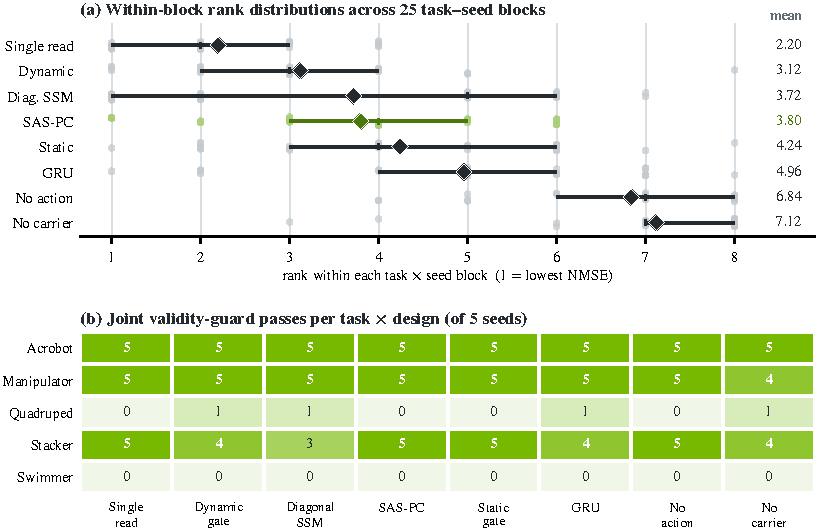
\includegraphics[width=\linewidth]{figures/fig_v18_task_design.pdf}
\caption{(a) Within-task, within-seed rank distributions for all eight designs; light points are the 25 task--seed ranks, bars span the interquartile range, ticks mark medians, diamonds mark mean rank, and rank 1 is the lowest NMSE within a block. SAS-PC is highlighted only to locate the candidate; ranks are descriptive, pool no raw NMSE across tasks, and define no superiority test. (b) Joint validity-guard passes per task and design (of five seeds), showing that guard failures are task-structured rather than design-specific.}
\label{fig:fig-v18-task-design}
\end{figure}

Exact rank summaries are:

\begin{table}[H]
\centering
\caption{Descriptive within-task, within-seed rank summaries corresponding to Figure \ref{fig:fig-v18-task-design}.}
\label{tbl:design-ranks}
\small
\begin{tabular}{@{}lrrrr@{}}
\toprule
\textcolor{NVIDIADark}{\textbf{Design}} & \textcolor{NVIDIADark}{\textbf{Mean rank}} & \textcolor{NVIDIADark}{\textbf{Median}} & \textcolor{NVIDIADark}{\textbf{First}} & \textcolor{NVIDIADark}{\textbf{Top-3}} \\
\midrule
Single read & 2.20 & 2 & 10/25 & 20/25 \\
Dynamic & 3.12 & 3 & 3/25 & 18/25 \\
Diag. SSM & 3.72 & 5 & 7/25 & 12/25 \\
SAS-PC & 3.80 & 4 & 3/25 & 10/25 \\
Static & 4.24 & 4 & 1/25 & 9/25 \\
GRU & 4.96 & 5 & 1/25 & 5/25 \\
No action & 6.84 & 7 & 0/25 & 0/25 \\
No carrier & 7.12 & 7 & 0/25 & 1/25 \\
\bottomrule
\end{tabular}
\end{table}

The frozen recurrent-envelope identity counts by task are:

\begin{table}[H]
\centering
\caption{Recurrent-envelope identities selected on the primary metric and reused for deep, clean, task, and corruption slices.}
\label{tbl:recurrent-identities}
\small
\begin{tabular}{@{}lrr@{}}
\toprule
\textcolor{NVIDIADark}{\textbf{Task}} & \textcolor{NVIDIADark}{\textbf{GRU selected}} & \textcolor{NVIDIADark}{\textbf{SSM selected}} \\
\midrule
Acrobot & 0/5 & 5/5 \\
Manipulator & 2/5 & 3/5 \\
Quadruped & 5/5 & 0/5 \\
Stacker & 0/5 & 5/5 \\
Swimmer-15 & 3/5 & 2/5 \\
\bottomrule
\end{tabular}
\end{table}

Condition-specific component effects and equal-condition phase slices
provide secondary context for Figure \ref{fig:fig-v18-secondary}:

\begin{table}[H]
\centering
\caption{Descriptive corruption-specific component effects. Positive values favor full SAS-PC; no multiplicity correction or decision gate is defined.}
\label{tbl:secondary-components}
\small
\begin{tabular}{@{}lrrr@{}}
\toprule
\textcolor{NVIDIADark}{\textbf{Corruption}} & \textcolor{NVIDIADark}{\textbf{vs no carrier}} & \textcolor{NVIDIADark}{\textbf{action transport}} & \textcolor{NVIDIADark}{\textbf{joint read}} \\
\midrule
Freeze & +10.91\% & +9.79\% & +0.50\% \\
Gaussian noise & +16.68\% & +10.48\% & -12.57\% \\
Checkerboard & +5.70\% & +5.30\% & -8.00\% \\
Long freeze & +10.11\% & +9.44\% & +1.65\% \\
\bottomrule
\end{tabular}
\end{table}

\begin{table}[H]
\centering
\caption{Descriptive phase effects against the primary-selected GRU/SSM identity, averaged equally across corruptions. Deep gap is nested within whole gap; intervals are unadjusted and define no decision gate.}
\label{tbl:secondary-phases}
\small
\begin{tabular}{@{}lrr@{}}
\toprule
\textcolor{NVIDIADark}{\textbf{Phase}} & \textcolor{NVIDIADark}{\textbf{Effect [95\% CI]}} & \textcolor{NVIDIADark}{\textbf{Cell/task wins}} \\
\midrule
Whole gap & +1.58\% [-7.60\%, +11.20\%] & 13/25; 3/5 \\
Deep gap & -1.74\% [-12.95\%, +9.46\%] & 11/25; 2/5 \\
First post-gap & -4.42\% [-15.80\%, +7.04\%] & 10/25; 1/5 \\
Post-gap & +8.27\% [+4.75\%, +12.86\%] & 23/25; 5/5 \\
\bottomrule
\end{tabular}
\end{table}

Per-corruption and per-phase values remain in each cell's
\texttt{metrics.json} and held-out rollout arrays. The paper does not
pool raw task-state MSE across heterogeneous tasks.

\section{Representation and
convergence}\label{representation-and-convergence}

\begin{table}[H]
\centering
\caption{Representation-health receipts by design.}
\label{tbl:representation-by-design}
\small
\begin{tabular}{@{}lrrrr@{}}
\toprule
\textcolor{NVIDIADark}{\textbf{Design}} & \textcolor{NVIDIADark}{\textbf{Min. variance}} & \textcolor{NVIDIADark}{\textbf{Min. rank}} & \textcolor{NVIDIADark}{\textbf{Variance pass}} & \textcolor{NVIDIADark}{\textbf{Rank pass}} \\
\midrule
No carrier & 0.0296 & 2.92 & 25/25 & 18/25 \\
GRU & 0.0230 & 2.02 & 25/25 & 17/25 \\
Diag. SSM & 0.0309 & 3.81 & 25/25 & 19/25 \\
SAS-PC & 0.0228 & 2.02 & 25/25 & 18/25 \\
No action & 0.0233 & 2.03 & 25/25 & 18/25 \\
Single read & 0.0245 & 2.38 & 25/25 & 18/25 \\
Static & 0.0349 & 4.62 & 25/25 & 18/25 \\
Dynamic & 0.0233 & 2.02 & 25/25 & 18/25 \\
\bottomrule
\end{tabular}
\end{table}

\begin{table}[H]
\centering
\caption{Late-window convergence receipts by design.}
\label{tbl:convergence-by-design}
\small
\begin{tabular}{@{}lrr@{}}
\toprule
\textcolor{NVIDIADark}{\textbf{Design}} & \textcolor{NVIDIADark}{\textbf{Largest late change}} & \textcolor{NVIDIADark}{\textbf{Convergence pass}} \\
\midrule
No carrier & +39.38\% & 15/25 \\
GRU & +43.71\% & 15/25 \\
Diag. SSM & +47.70\% & 16/25 \\
SAS-PC & +90.25\% & 15/25 \\
No action & +132.09\% & 17/25 \\
Single read & +120.28\% & 15/25 \\
Static & +36.58\% & 17/25 \\
Dynamic & +47.34\% & 16/25 \\
\bottomrule
\end{tabular}
\end{table}

Representation health requires both thresholds to be met in every cell.
Convergence is the absolute relative change between mean validation
predictive loss over epochs 81--90 and 91--100. The gate requires every
cell's late change to be at most 5\%; no failing arm is removed.

\section{Integrator guard}\label{integrator-guard}

For target \(t\), the legal feature vector is \([E_\theta(o_0),a_{t-3:t-1},\sum_{j=0}^{t-1}a_j,t/(L-1)]\),
with zero-padding before three actions exist. The candidate checkpoint
supplies \(E_\theta\); a ridge map is fit on clean training targets and
evaluated only on deep and first-post held-out samples. The integrator
receives no observation after the visible \(o_0\).

\begin{table}[H]
\centering
\caption{Legal initial-frame/action integrator guard by task. Positive paired reduction favors SAS-PC.}
\label{tbl:integrator-guard}
\small
\begin{tabular}{@{}lrrrr@{}}
\toprule
\textcolor{NVIDIADark}{\textbf{Task}} & \textcolor{NVIDIADark}{\textbf{SAS-PC prior NMSE}} & \textcolor{NVIDIADark}{\textbf{Integrator NMSE}} & \textcolor{NVIDIADark}{\textbf{Paired reduction}} & \textcolor{NVIDIADark}{\textbf{Seed wins}} \\
\midrule
Acrobot & 0.572 & 0.416 & -37.45\% & 0/5 \\
Manipulator & 0.959 & 0.821 & -16.74\% & 0/5 \\
Quadruped & 1.097 & 0.618 & -77.40\% & 0/5 \\
Stacker & 0.930 & 0.802 & -15.91\% & 0/5 \\
Swimmer-15 & 0.890 & 0.622 & -43.14\% & 0/5 \\
\bottomrule
\end{tabular}
\end{table}

\section{Adaptive provenance and
restart}\label{adaptive-provenance-and-restart}

SAS-PC was selected after V1--V7 development on different tasks. Its
earlier adaptive V8 study completed 325 cells but had immutable label
\texttt{PILOT\_NO\_GO\_FINAL\_DESCRIPTIVE}; it cannot rescue the present
confirmation (V18). V9--V17 are likewise development/host audits, not
confirmation. Interruption 1,
\texttt{acrobot.swingup/vicreg\_ssm/s18005}: last interrupted epoch 62;
interrupted/replacement log hashes
\texttt{dfe369fac5d9}/\texttt{de69a7091d8a}; replacement epochs 1--100.
Interruption 1, \texttt{manipulator.bring\_ball/vicreg\_ssm/s18005}:
last interrupted epoch 31; interrupted/replacement log hashes
\texttt{3492682adbf9}/\texttt{2c516e0b6f8c}; replacement epochs 1--100.
Interruption 1, \texttt{quadruped.run/vicreg\_ssm/s18005}: last
interrupted epoch 9; interrupted/replacement log hashes
\texttt{6a72339d3e8e}/\texttt{6f005ea3ae51}; replacement epochs 1--100.
Interruption 1, \texttt{swimmer.swimmer15/vicreg\_ssm/s18005}: last
interrupted epoch 62; interrupted/replacement log hashes
\texttt{4029c6a1b1be}/\texttt{5e0815242313}; replacement epochs 1--100.
Interruption 2,
\texttt{stacker.stack\_4/vicreg\_hacssmv8\_static/s18003}: last
interrupted epoch 37; interrupted/replacement log hashes
\texttt{e74f6ba0dcb1}/\texttt{63b9ee95f0eb}; replacement epochs 1--100.
The runner's JSON attempts ledger records terminal subprocess returns,
so process-killed attempts are supplied by this independently verified
schema-v2 lineage receipt. The audit's separately classified parent-only
pause did not signal the trainer and is not counted as an additional
restart. The registered commands, seeds, source hashes, and stopping
rule were unchanged.

\section{Claim boundary}\label{claim-boundary}

The study can establish only a persistent-state or
component-intervention result for a VICReg-trained LeWM-derived
finite-context host on the frozen corruption cohort. It cannot establish
improvement to original SIGReg LeWM, executed-return or planning gains,
causal discovery, learned semantic hierarchy, calibrated uncertainty,
learned horizon discovery, or robustness beyond these tasks and
corruptions.

\section{LLM Usage Statement}\label{llm-usage-statement}

OpenAI Codex assisted with code review, experiment monitoring, artifact
auditing, deterministic result-to-manuscript tooling, and manuscript
drafting/editing. The authors verified the executed code, artifacts,
statistics, citations, and final claims and retain responsibility for
the work.
